\documentclass[UTF8]{ctexart}
\usepackage[left=3.2cm,right=3.2cm,top=2.33cm,bottom=2.33cm]{geometry}
\usepackage{fancyhdr}
\usepackage{graphicx}
\pagestyle{fancy} 
\rhead{\sf Machine Learning}		% 标题
\cfoot{\thepage}
\rfoot{\color{gray}\tt SVM}
\usepackage[svgnames]{xcolor}
\usepackage{hyperref}
\setlength\parskip{.3\baselineskip}
\hypersetup{
	%   bookmarks=true,     	% show bookmarks bar?
	%   CJKbookmarks=true,     	% 中文支持
	unicode=true,          	% non-Latin characters in Acrobat’s bookmarks
	pdftoolbar=true,        	% show Acrobat’s toolbar?
	pdfmenubar=true,        	% show Acrobat’s menu?
	pdffitwindow=false,     	% window fit to page when opened
	pdfstartview={FitH},    	% fits the width of the page to the window
	%pdftitle={My title},    % title
	%pdfauthor={Author},     % author
	%pdfsubject={Subject},   % subject of the document
	%pdfcreator={Creator},   % creator of the document
	%pdfproducer={Producer}, % producer of the document
	%pdfkeywords={keywords}, % list of keywords
	%pdfnewwindow=true,      % links in new window
	colorlinks=true,         % false: boxed links; true: colored links
	linkcolor=Black,		  	% color of internal links
	citecolor=Magenta,      	% color of links to bibliography
	filecolor=green,        	% color of file links
	urlcolor=DarkBlue       	% color of external links
}
\usepackage{enumerate}
\usepackage{amssymb, amsmath, mathrsfs, mathtools}
\usepackage{amsthm}
\usepackage{listings}
\lstset{
	numbers = left, % 想要代码行号请反注释这一行
	numberstyle = \small\ttfamily,
	frame = shadowbox,
	basicstyle = \ttfamily \bfseries,
	keywordstyle = \color{blue!70},
	commentstyle = \color{red!50!green!50!blue!50}, 
	rulesepcolor= \color{red!20!green!20!blue!20},
	xleftmargin = 0.3em,
	xrightmargin = 0.5em,
	% aboveskip = 1em
} 
% \lstset{numbers=left, frame=shadowbox, basicstyle=\ttfamily, commentstyle=\fontseries{lc}\selectfont\slshape, columns=fullflexible, breaklines=true, escapeinside={(*@}{@*)}} % From LM
\newtheorem{lemma}{引理}
\begin{document}
	\begin{titlepage}
		\vspace*{\fill}
		\begin{center}
			\normalfont
			{\Huge \bfseries 机器学习上机报告}
			
			\bigskip
			
			{\Large \itshape 林远钊 1700010672}
			
			\medskip
			
			\today
		\end{center}
		\vspace{\stretch{3}}
	\end{titlepage}
	\newpage
	\tableofcontents
	
	\newpage
\section{支持向量机Review}
\paragraph{基本介绍}支持向量机(Support Vector Machines, SVM)是一种监督学习的方法,可用于分类,回归和异常值探查。其优点包括:在高维空间效率较高,在维数高彧样本数时仍然有效,可以用总体训练数据中的一部分(称为“支持向量”)的一部分来生成决策函数(这意味着它的存储性能是比较好的);而它的缺点有:如果特征的数目远大于样本的数目,那么合理的选择核函数和正则化项是重要而困难的,而且支持向量机不直接给出概率估计。

\paragraph{实现工具}本次上机作业中主要通过scikit-learn这一python包来实现支持向量机。在使用之前需要对其进行一定的了解和学习。

sklearn(scikit-learn包的常用缩写)中有专门的svm模块,可以通过命令
\begin{lstlisting}[language= python]
from sklearn import svm
\end{lstlisting}
导入该模块,本次上机中使用到的主要是其中的支持向量分类器(SVC)和支持向量回归(SVR)。

\newpage
\section{python实现}
由于本次上机中使用了包,大可把其作为黑箱,其中具体实现细节不必深究。

\subsection{数据格式}
同上一次对数据的处理一样,在处理书中所给表格3.0$\alpha$中的数据时,我们将数据处理为.csv文件形式,第一行为数据的属性集合,以下每行对应一个数据在这些属性上的取值。好瓜的标签(label)记作1,坏瓜则记为-1。

\subsection{实现思路}
首先需要先将所给数据转化成易于处理的形式。这里我们利用numpy和pandas包中的方法进行简单的转化,相应定义一个信息处理函数loadData(filename)
\begin{lstlisting}[language = python]
"""默认csv文件第一行是列属性,以下每行是训练数据
并且数据的最后一列必然是数据的label"""
frame = pd.read_csv(filename)#读为DataFrame格式
labels = frame['label']#获取标记
attrset = list(frame.columns)
attrset.remove('label')
dataset = list(frame.values)
for i in range(frame.shape[0]):#遍历所有数据
	dataset[i] = list(dataset[i])
	dataset[i].pop()
return dataset, list(labels), attrset
#返回数据集(Dataset)和标记集(List)和属性集
\end{lstlisting}

\subsection{支持向量分类SVC}
为了回答6.2中的问题,分别使用线性核和高斯核训练一个SVM
\begin{lstlisting}[language=python]
dataset, labels, attrset = loadData('data3.0alpha.csv')
kernel = ('linear', 'rbf')
clf1 = svm.SVC(kernel='linear')
clf2 = svm.SVC(kernel='rbf', gamma='scale')

ans = (clf1.fit(dataset, labels), clf2.fit(dataset, labels))

for i in range(2):
	svs = ans[i].support_vectors_
	print('核函数为',kernel[i],'的支持向量为:')
	for j in range(len(svs)):
		print(svs[j])
	print('支持向量的个数为',len(svs))
\end{lstlisting}

输出结果依次被记录在以下的两个图中(已进行可视化处理)。附件中有原图和纯数据的输出。

\begin{figure}[htbp]
	\centering
	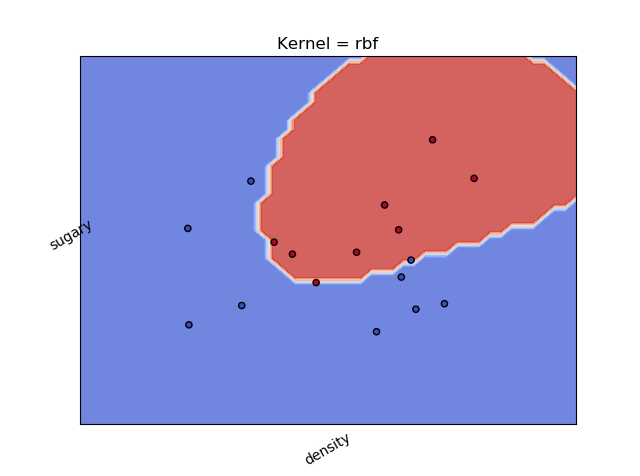
\includegraphics[scale=0.5]{RBF.PNG}
	\caption{RBF}
\end{figure}
\begin{figure}[htbp]
	\centering
	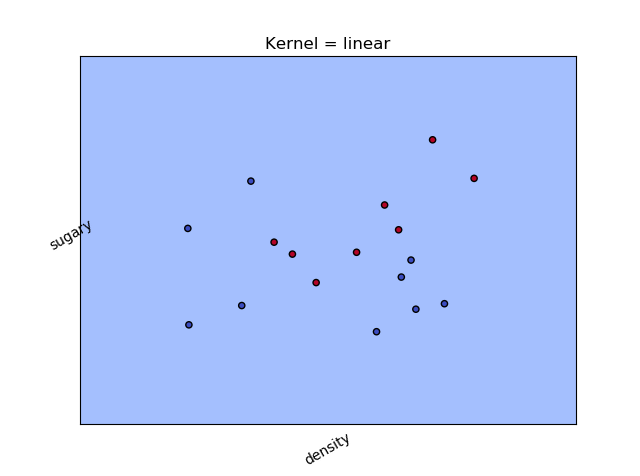
\includegraphics[scale=0.5]{Linear.PNG}
	\caption{Linear}
\end{figure}

可以看到高斯核的预测性质似乎更为合理,而线性核则只能做到将全平面分为一类,这说明线性核对于这个问题是极其不适用的。其中线性核的支持向量是16个,而高斯核支持向量是17个。
(ps:私以为本题中数据数量过少应该也是分类效果不佳的原因之一)
\subsection{关于支持向量数目的讨论}
显然,总样本数只有17个,习得的支持向量数却分别有16、17个,这件事情不是那么的令人满意。笔者在这个问题上犹豫了很久,最后发现如果将参数max\_iter 设定为一些值(如1),
可以显著减少支持向量个数(减少到只有2个)。原因是max\_iter是SMO算法的迭代次数,当不限制迭代次数时,训练出的模型会和给定样本更加贴合(当然有过拟合的风险),介于此,
在上面并未刻意调整支持向量个数,而保留了最开始的结果。

\subsection{支持向量回归SVR}
为了回答6.8中的问题,调用svm.SVR类即可得
\begin{lstlisting}[language = python]
frame = pd.read_csv('data3.0alpha.csv')
labels = frame['label']
X = frame['密度']
Xm = []
for x in X:
	Xm.append([x])
y = frame['含糖率']
clf = svm.SVR(gamma='scale',kernel='rbf')
clf.fit(Xm, y)
\end{lstlisting}
即可得到SVR。

\section{对支持向量的优化}
基于一个朴素的想法:在进行支持向量分类前先对数据进行某种预处理,使得样本点中有极大相似性的部分被合理地替代,在这一步处理便尽量不丢失信息地减少样本点的数量,尤其是非支持向量的个数,由此减少支持向量的数量而不显著地降低SVM的泛化性能。

具体实现中,采用聚类(Cluster)的技术来达到以上所述的目的,并且以下通过对iris数据集的分析来粗略地了解该技术的效果。
\subsection{聚类(Clustering)简介}
聚类是一种无监督学习的方法。

在sklearn中,每个聚类算法主要都有两种形式,一种是一个类,其中的方法fit可以习得训练数据的聚类;亦或者是一个函数,在给定训练数据时,返回一个整数标记的数组对应着不同的聚类。简单地,以下采用K-均值法进行聚类学习。

基本思想是:在给定数据后,将数据依原类别分开,并对分开后的若干组数据分别做KMeans聚类学习,得到学习后的每组聚类均值点。以这些均值点作为新的数据依据进行学习。当然,以上聚类学习学得类的数目是一个应当调整的参数。

\subsection{具体试验}
以下将以iris数据集为例,观察之前策略的学习效果。

在sklearn官方文档中给出了对iris数据集分别以四种不同核函数学习的结果如下图所示。
\begin{figure}[htbp]
	\centering
	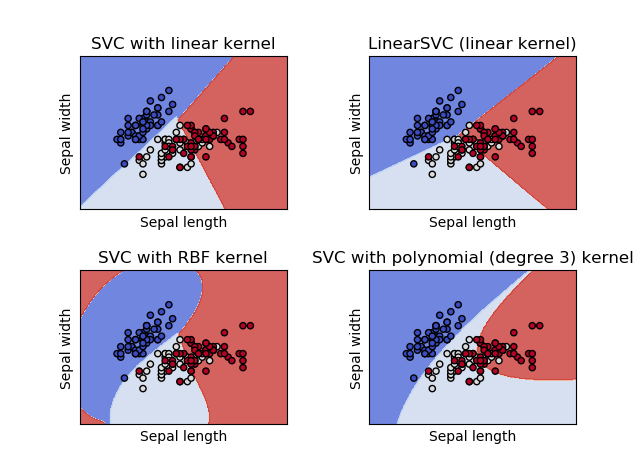
\includegraphics[scale=0.8]{iris_before.PNG}
	\caption{iris-before}
\end{figure}

而iris数据集中共有150个数据,每种类别的数据各有50个,因而对每一个类别中的数据进行聚类学习,保留10个聚类均值数据作为新的数据依据进行学习。得到新的结果如下。
\begin{figure}[htbp]
	\centering
	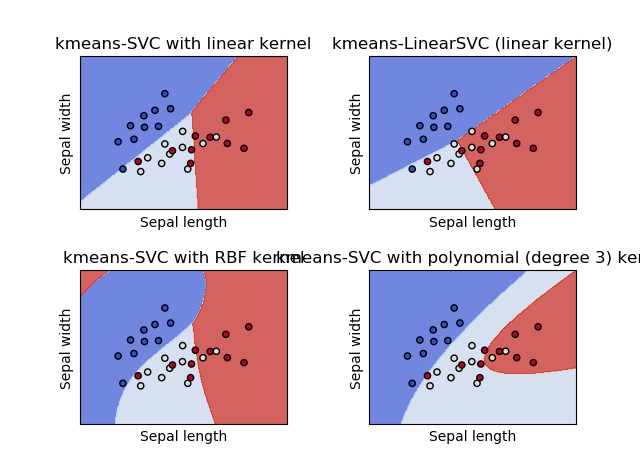
\includegraphics[scale=0.8]{iris_after.PNG}
	\caption{iris-after}
\end{figure}

可以看到习得的模型并无显著改变且显然支持向量数将减少(样本数减少到之前的1/10)。
以上便是6.10的解答。

附件中包含了报告中所有的图片及使用的所有源代码。

(PS:Latex水平比较差,最后图片部分排版炸了qwq 助教见谅)
\end{document}
